\documentclass{article}

% E&D track, anonymous submission
\usepackage[eandd]{neurips_2026}

\usepackage[utf8]{inputenc}
\usepackage[T1]{fontenc}
\usepackage{hyperref}
\usepackage{url}
\usepackage{booktabs}
\usepackage{amsfonts}
\usepackage{amsmath}
\usepackage{nicefrac}
\usepackage{microtype}
\usepackage{xcolor}
\usepackage{graphicx}
\usepackage{multirow}
\usepackage{longtable}
\usepackage{float}

% suppress overfull hbox warnings below 5pt
\hfuzz=5pt

\title{Beyond Energies and Forces: OMol-Descriptors-4M, an Open
  Post-DFT Pipeline and Evaluation Protocol for Machine Learning in Chemistry}

\author{%
  Santiago Vargas \\
  Chemical Science Division \\
  Lawrence Berkeley National Laboratory \\
  \texttt{SantiagoVargas@lbl.gov} \\
  \And
  Samuel M. Blau \\
  Energy Technologies Area \\
  Lawrence Berkeley National Laboratory \\
  \texttt{smblau@lbl.gov} \\
}

\begin{document}

\maketitle

\begin{abstract}


We present \texttt{generator}, an end-to-end computational chemistry
post-analysis framework that processes repositories of molecular DFT wavefunctions
and yields six partial-charge schemes (Hirshfeld, CM5, ADCH, Becke, Mulliken, Loewdin), 
four bond-order schemes, full QTAIM
topology, fuzzy descriptors, and ORCA-derived globals. We built this by
wrapping per-tier analysis routines around Multiwfn and ORCA's \texttt{orca\_2mkl}
utility, packaging the result into a scalable workflow for HPC clusters.
Users can select compute tiers to trade fidelity for cost, then compact
the resulting calculations into portable sharded Lightning Memory-Mapped
Databases (LMDBs) keyed by job identity for downstream analysis and
machine learning.
To demonstrate the pipeline, we processed the recently-released OMol25
electronic structure dataset: a 4M-structure public subset of the
110M+-calculation 2025 release that ships the complete DFT outputs,
including density matrices, energy gradients, ORCA \texttt{.out} files, and
\texttt{.gbw} wavefunctions. By post-processing the wavefunctions, we extract
atom-, bond-, and molecule-level descriptors across $\sim$4M structures
spanning 34 chemical verticals, supplementing the original dataset's energy
and force labels with physically-interpretable quantities.
We name this dataset OMol-Descriptors-4M and present it as the first
multi-vertical descriptor dataset at this scale beyond energies and forces.
Analogous to the source dataset, we establish an evaluation protocol with
explicit evaluative claims and scope boundaries: composition-ordered
train/val/test splits via blake2b-hashed molecular formula and five
domain-specific held-out stress tests (metal-ligand bond pairs, lanthanide-ligand
bond pairs, reactivity, large systems, and high-charge regimes; $\sim$60k
structures total). Together with the open
generation pipeline, these components let researchers reuse the protocol
on new wavefunction repositories across molecular chemistry.

\end{abstract}

\section{Introduction}
\label{sec:intro}
% Motivating gap: descriptor-based ML bottlenecked by O(10^3)-O(10^5) labeled datasets.
% Three-claim structure: Scale, Pipeline, Evaluation.
% Track-fit paragraph: explicit evaluative claims, scope, what the dataset cannot evaluate.
% Final paragraph: contributions list.

Machine learning and deep learning have upended the relationship between large datasets
and how we interpret, predict, and generate information.
Prior to this revolution, humans relied on low-dimensional embeddings and descriptors to 
parse and understand large swaths of data. Today, a wide spectrum of models operate on language~\citep{gpt3},
vision~\citep{yolo,sam}, and biological~\citep{alphafold2} data. In the chemical sciences, we have seen the decades long
development of descriptors and models heat up in the last 10 years. Cheminformatics via 
fingerprinting descriptors \citep{ecfp} and Morgan~\citep{morgan1965} coupling to tree-based supervised-learning algorithms\cite{ahneman2018}
have given way to advanced architectures and representations rooted in graph-based embeddings 
of chemical structures. These newer approaches include continuous-filter graph neural
networks~\citep{schnet}, directional message-passing architectures~\citep{dimenetpp},
and equivariant foundation models capable of stable atomistic simulation across
nearly the entire periodic table~\citep{macemp}. High-profile applications include
generative inorganic materials design with MatterGen~\citep{mattergen}, the OMat24
dataset and models for materials neural network potentials~\citep{omat24}, and 3D
pre-training on hundreds of millions of conformers for broad molecular property
prediction~\citep{unimol}.



Naturally, chemistry and material science, with their mature methods for generating simulated data via
Density Functional Theory (DFT) have led to the creation of many datasets. QM9, for example, is one of the
most popular datasets and covers a set of $\sim$134K organic molecules with up to 9 heavy atoms~\citep{qm9}.
Beyond this, SPICE~\citep{spice} and ANI-1x~\citep{ani1x} extended this coverage to biomolecular and reactive domains. OC20~\citep{oc20}, Materials Project~\citep{matproj}
and tmQM+~\citep{D5DD00220F} pushed the boundary towards inorganic materials and transition-metal complexes. Alongside datasets, benchmarking suites such as
MoleculeNet~\citep{moleculenet} and MOSES~\citep{moses} have standardized
evaluation across property prediction and molecular generation tasks. The recent OMol25~\citep{levine2026openmolecules2025omol25} is notable among molecular MLIP datasets due to 
its size, diversity, and high-level of accuracy. It pushes beyond 100M structures, 
80+ elements, and many chemical verticals to provide the community with a rich repository for 
training neural network potentials. To date, the team has shared the wavefunction, density matrices, 
and orca.out files of 4M of those datapoints. This additional information serves as the basis for this work 
where we post-processed OMol25 wavefunctions to yield a new dataset of descriptors. 
We name the result \textbf{OMol-Descriptors-4M} and contribute: (i) the dataset
itself, (ii) the open generation pipeline, and (iii) an evaluation protocol with
composition-ordered splits, five held-out stress-test suites, and quantified
per-descriptor noise floors.

\section{Related Work}
\label{sec:related}

Descriptor-rich quantum-chemistry datasets divide along two axes: the
chemical envelope they cover and the descriptor families they incorporate.
Smaller, single-purpose releases such as QM9, QMugs, OE62, BDE-db, and
tmQM+ \citep{qm9, qmugs, oe62, bdedb, D5DD00220F} sit below $10^{6}$
structures and typically contain only one descriptor family per dataset.
In contrast, modern force-field training corpora such as ANI-1x/2x, SPICE, GEOM,
transition1x, and OMol25 itself \citep{ani1x, ani2x, spice, geom,
transition1x, levine2026openmolecules2025omol25} routinely
cross $10^{6}$--$10^{8}$ structures but focus only on energies, forces, and
occasionally, a limited set of other features. Even when the latter contain information such as dipoles,
orbital information, and/or partial charges, they typically use only one or two cruder schemes.
OMol-Descriptors-4M encompasses a wider diversity and size vs. existing descriptor datasets, all 
while providing far more descriptors as compared to existing datasets for training MLIPs. 
As this is a broader descriptor dataset, we will only use comparators with a wider 
set of features beyond one partial charge scheme that are also not contained within the 
larger OMol25 dataset. 


\subsection{Comparable-scale descriptor comparators}
\label{sec:related-comparators}

As mentioned, any comparison of descriptors between our dataset and others is moot as existing datasets simply do not cover the diversity
of features within OMol-Descriptors-4M, and typically, do not contain the chemical diversity of OMol25. In lieu of this, we opted to compare
the structural diversity within our dataset to others of comparable descriptor richness, namely, QM7-X, SchNet4AIM, and tmQM+.
QM7-X \citep{qm7x} reaches 4.2M conformers with a rich per-atom data
inventory: Hirshfeld charges, dipoles, atomic $C_{6}$ coefficients,
polarizabilities, van der Waals radii, and a PBE0+MBD energy
decomposition -- but only 6{,}950 unique compositions across CHNOSCl compositions
with at most seven heavy atoms. SchNet4AIM\citep{schnet4aim}, though smaller with only $\sim$3.8K structures, is a closer
analog on the axis of dataset diversity. It contains only CHNO atoms but incorporates QTAIM charges, 
atomic localization indices ($\lambda$), and pairwise
delocalization indices ($\delta$). The tmQM+ dataset \citep{D5DD00220F} is a near precedent on the
descriptor-richness axis for transition-metal chemistry: it incorporates
$\sim$60{,}000 transition-metal complexes with full QTAIM topology
(critical-point scalars, Lagrangian and Hamiltonian kinetic energy
densities, electron localization function, ESP components, gradient and
Laplacian norms, ellipticity, and pairwise QTAIM bond indices) computed
at three levels of theory. 


\begin{table}[h]
\centering
\footnotesize
\setlength{\tabcolsep}{3pt}
\caption{Comparator datasets used for the structural-overlap audit.
``Compositions'' counts unique molecular formulas.}
\label{tab:comparators}
\begin{tabular}{lrrll}
\toprule
Dataset & Structures & Compositions & Chemical Vertical & Descriptors \\
\midrule
QM7-X        & 4.2M  & 6.9k  & CHNOSCl, $\leq 7$ heavy atoms  & Hirshfeld; $C_{6}$, $\alpha$, vdW; PBE0+MBD \\
SchNet4AIM   & 3.9k  & 3.9k  & CHON                         & QTAIM $Q$, $\lambda$, $\delta$ \\
tmQM+~\citep{D5DD00220F}        & 60k   & 60k   &
  \begin{tabular}[t]{@{}l@{}}3d/4d/5d transition-metal \\ complexes \end{tabular} &
  \begin{tabular}[t]{@{}l@{}}Full QTAIM topology, ELF, ESP, \\ kinetic energy densities; 3 LOTs\end{tabular} \\
\midrule
\textbf{Ours} & \textbf{4.0M} & \textbf{1.30M} &
  \begin{tabular}[t]{@{}l@{}}TM, charged, \\ reactive, protein-derived\end{tabular} &
  \begin{tabular}[t]{@{}l@{}}6 charge, 4 bond-order schemes, \\ full QTAIM, fuzzy, ORCA globals\end{tabular} \\
\bottomrule
\end{tabular}
\end{table}

%\subsection{Structural overlap}
%\label{sec:related-overlap}

We confirm that the descriptor breadth above corresponds to genuine
chemistry-space coverage by projecting OMol-Descriptors-4M against the
organic comparators in SOAP-UMAP space (Fig.~\ref{fig:umap_coverage}). The
embedding is fit on a balanced 500-molecule-per-source anchor (1{,}500
points total) using a 6-element common species set
(H, C, N, O, S, Cl). The TM-side overlap with tmQM+ requires a
TM-inclusive SOAP basis and is reported separately in
App.~\ref{app:umap_omol_vs_tmqmplus} where we see that, again, OMol-Descriptors-4M
appears to cover a superset of chemical structures.

\begin{figure}[h]
\centering
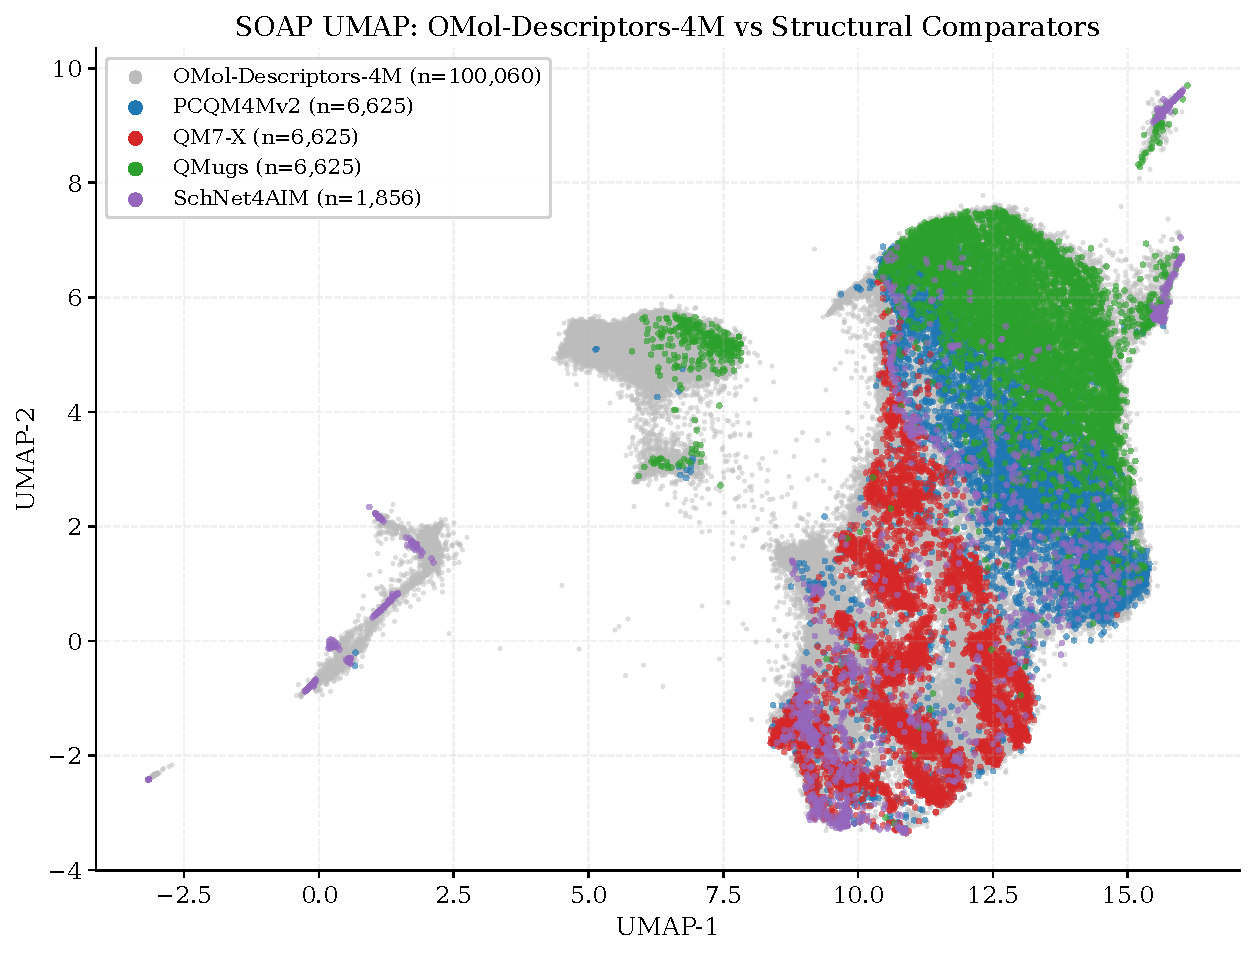
\includegraphics[width=\textwidth]{figures/umap/umap_all_paper.pdf}
\caption{SOAP-UMAP embedding of OMol-Descriptors-4M against the two
organic structural comparator datasets. Each point is a molecule projected via
UMAP fitted on a 500-molecule-per-source balanced subsample. SOAP descriptors use a
6-element species set
(H, C, N, O, S, Cl) common to all three sources.
OMol-Descriptors-4M (gray) is rendered as a background haze to expose
the relative positions of QM7-X and SchNet4AIM.}
\label{fig:umap_coverage}
\end{figure}

\section{Dataset}
\label{sec:dataset}


\subsection{Descriptor Families}

\textbf{Partial charges.}
Six independent atomic partial-charge schemes are computed per structure.
Hirshfeld \citep{hirshfeld1977}, CM5 \citep{cm5}, ADCH \citep{adch}, and Becke
\citep{becke1988} charges are produced by Multiwfn \citep{multiwfn} from the DFT electron density;
Mulliken and L\"owdin charges are extracted directly from the ORCA output \citep{orca5}.
Hirshfeld charges partition the electron density by the stockholder principle: each
atom claims a share of the density at every point proportional to its free-atom
promolecular density, yielding compact, chemically intuitive atomic populations.
CM5 applies a pairwise connectivity-based correction to Hirshfeld charges to
reproduce experimental dipole moments across diverse environments \citep{cm5}.
Becke charges integrate the molecular density over smooth, fuzzy atomic basins
defined by Becke's numerical weight functions \citep{becke1988}, providing a
partition that is independent of the basis set and free of the basis-function
artifacts that affect Mulliken and L\"owdin populations.
ADCH further corrects Hirshfeld charges for atomic dipole contributions to reduce
basis-set dependence \citep{adch}.

\textbf{Bond orders.}
Four schemes are universal across the corpus: Mayer \citep{mayer1983} and
L\"owdin bond orders from ORCA, fuzzy bond orders from Multiwfn
\citep{multiwfn,becke1988}, and QTAIM bond presence inferred from bond critical points.
Mayer bond orders derive from the density matrix and capture bond multiplicity
beyond formal valence, including partial and dative character.
L\"owdin bond orders use a symmetrically orthogonalized basis, reducing
the basis-set sensitivity that affects Mulliken-derived indices.
Fuzzy bond orders integrate the exchange-correlation hole over Becke fuzzy-atom
basins, providing a real-space, basis-set-independent measure of covalent
bond character. QTAIM bond presence is a binary signal at each bond critical
point; the corresponding density and Laplacian scalars are stored under QTAIM topology.

\textbf{QTAIM topology.}
Critical points of the electron density are located via Multiwfn following Bader's
Quantum Theory of Atoms in Molecules \citep{bader1990}.
Each bond critical point carries 26 scalar fields ($\rho$, $\nabla^2\rho$,
ellipticity, kinetic/potential energy densities); ring and cage CPs, non-nuclear
attractors, and atomic basin integrals are stored where present.

\textbf{Fuzzy and surface descriptors.}
Fuzzy atom analysis partitions molecular properties via smooth, overlapping atomic
weight functions, yielding basis-set-independent atomic populations, valences, and
bond orders~\citep{mayersalvador2004}.
Per-atom Becke and Hirshfeld fuzzy electron-density integrations \citep{becke1988}
are computed via Multiwfn for every structure (with spin-density counterparts for
open-shell records).
These provide atomic electron and spin populations that are independent of the
one-electron basis. Molecular-level ALIE (Average Local Ionization Energy) 
surface properties, including surface volume, area, extrema, polarity index, 
and internal charge separation are additionally extracted per molecule, 
encoding site-specific electrophilicity and reactivity complementary 
to the atomic-level descriptors.

\textbf{ORCA globals.}
Total SCF energy, HOMO/LUMO orbital energies, molecular dipole, nuclear gradient, and
SCF convergence metadata are parsed from the ORCA output file \citep{orca5,ORCA}.


\subsection{Storage Layout}
\label{sec:storage}

Each split folder contains eight LMDB files keyed on a single string identifier
$k = \texttt{relpath(folder, root).replace("/", "\_\_")}$. Keys for each structure
are shared across all lmdbs and they each contain different datatypes:
\begin{itemize}
\item \texttt{structure.lmdb}: pymatgen \texttt{Molecule} (positions, elements), total spin and charge, RDKit-derived bond list, and external identifiers.
\item \texttt{charge.lmdb}: per-atom charges nested by scheme (\texttt{hirshfeld}, \texttt{cm5}, \texttt{adch}, \texttt{becke}, \texttt{mulliken\_orca}, \texttt{loewdin\_orca}); \texttt{hirshfeld}/\texttt{cm5} also carry a total dipole, \texttt{adch}/\texttt{becke} carry total and per-atom dipoles.
\item \texttt{qtaim.lmdb}: per-structure dict of critical points keyed by atom ID for nuclear CPs or by atom-pair for bond CPs; 26 scalar fields per CP including $\rho$, $\nabla^{2}\rho$, ellipticity, kinetic and potential energy densities.
\item \texttt{bond.lmdb}: bond-order schemes (\texttt{fuzzy\_bond}, \texttt{mayer\_orca}, \texttt{loewdin\_orca}) keyed by directed atom-pair strings \texttt{"\{i\}\_\{El\_i\}\_to\_\{j\}\_\{El\_j\}"}; the fourth scheme, QTAIM bond presence, is recoverable from \texttt{qtaim.lmdb} BCP keys.
\item \texttt{fuzzy.lmdb}: per-atom Multiwfn fuzzy integrations (\texttt{becke\_fuzzy\_density}, \texttt{hirsh\_fuzzy\_density}; spin counterparts for open-shell records).
\item \texttt{other.lmdb}: molecular descriptors from ESP and ALIE surface analysis (volume, surface area, min/max, signed mean and variance, polarity index, internal charge separation) plus four polarity scalars (\texttt{mpp\_full}, \texttt{sdp\_full}, \texttt{mpp\_heavy}, \texttt{sdp\_heavy}).
\item \texttt{orca.lmdb}: ORCA-derived globals (total energy, orbital energies, dipole, gradient, SCF metadata), filtered via \texttt{DEFAULT\_ORCA\_FILTER} when consumed by the converter.
\item \texttt{timings.lmdb}: per-job step durations; provenance only.
\end{itemize}


\subsection{Data Quality and Per-Vertical Breakdown}
\label{sec:dataset-quality}

Calculations and conversions to LMDBs are highly stable with five of the
seven analytic LMDBs showing no corrupt or incomplete data storage. 
For \texttt{qtaim} and \texttt{orca} we have 25 (0.0006\%) and 1{,}607 (0.0403\%)
failed calculations; the ORCA failures concentrate on physically
hard cases (solvated biomolecules, scaled-separation electrolytes,
open-shell TM redox), and geometry plus Multiwfn-side descriptors stay
valid for those records. The failed QTAIM records were instances where
no BCPs were detected or where the Poincare-Hopf formula was not obeyed.
Cross-LMDB key alignment holds to within four
records on a 4M-key index, so any descriptor combination joins on
the full corpus. Each of the six charge schemes (Hirshfeld, ADCH, CM5,
Becke, Mulliken, L\"owdin), four bond-order schemes (fuzzy,
Mayer, L\"owdin, QTAIM), full QTAIM topology, and the standard ORCA globals
reaches $\geq$99\% on every one of the 34 verticals; in other words, the same
profile is available for a noble-gas dimer, a 200-atom solvated protein
pocket, and a transition-metal redox complex. Full audit
table, coverage heatmap, and per-vertical record counts:
App.~\ref{app:lmdb_audit} and Table~\ref{tab:t1_census}.

\section{Pipeline}\label{sec:pipeline}

\subsection{Architecture}
\begin{figure}[t]
  \centering
  \includegraphics[width=\linewidth]{figures/pipeline_diagram.png}
  \caption{Overview of the \texttt{generator} post-processing pipeline. Starting from an
    OMol25 \texttt{.gbw} wavefunction, the pipeline converts to Molden format (with EDF
    loading for ECP correctness), runs one of three calculation tiers through Multiwfn, and
    emits seven per-folder JSON outputs. These are converted to typed LMDBs sharing a common
    key, which can be consumed directly by graph-based frameworks or converted to DGL
    heterographs via our sister package \texttt{qtaim\_embed}\footnote{\url{https://github.com/santi921/qtaim_embed}}.}
  \label{fig:pipeline}
\end{figure}

The pipeline is an orchestration layer over two external binaries, ORCA's
\texttt{orca\_2mkl}~\cite{ORCA} and Multiwfn~\cite{multiwfn}, applied to the 4M OMol25
electronic-structure release that ships wavefunctions, density matrices, and raw ORCA
outputs (\texttt{.out}, \texttt{.engrad}, \texttt{orca\_property.txt}). For each job folder
we read the \texttt{.gbw} and \texttt{.out}; because Multiwfn has more complete
compatibility with \texttt{.wfn}/\texttt{.wfx} files, the \texttt{.gbw} is converted to
Molden via \texttt{orca\_2mkl} and the EDF library is loaded inside Multiwfn so ECPs are
treated correctly~\citep{multiwfn}. Folders that fail the EDF load are flagged
automatically (see Sec.~\ref{sec:dataset}) and re-queued.

A user selects a calculation tier through a single integer \texttt{full\_set}~$\in\{0,1,2\}$
which cascades through the four post-DFT families implemented in
\texttt{qtaim\_gen/source/data/multiwfn.py}. Tiers are strict supersets, so calculations
stack from 0 to 2 as descriptor needs grow. Table~\ref{tab:tiers} summarizes per-family
additions at each tier; the QTAIM critical-point search and ORCA-derived globals run at
every tier.

\begin{table}[H]
\centering
\small
\caption{Per-family contents of each calculation tier (\texttt{full\_set}). Tiers are
strict supersets: tier $k$ runs everything in tiers $0, \dots, k$. Schemes shown in a column
are those \emph{added} at that tier. Source: \texttt{qtaim\_gen/source/data/multiwfn.py}.}
\label{tab:tiers}
\begin{tabular}{lp{3.6cm}p{3.0cm}p{3.4cm}}
\toprule
\textbf{Family} & \textbf{Tier 0 (baseline)} & \textbf{Tier 1 (+adds)} & \textbf{Tier 2 (+adds)} \\
\midrule
Partial charges & Hirshfeld, ADCH, CM5, Becke & VDD, MBIS, CHELPG & Bader (basin-integrated) \\
Bond orders & Fuzzy bond order & IBSI bond order & Laplacian bond order \\
Fuzzy density & Becke density, Hirshfeld density, Becke spin, Hirshfeld spin & ELF, MBIS density, MBIS spin & Laplacian $\rho$, gradient-norm $|\nabla \rho|$ \\
Other (scalar fields) & Geometry (ellipticity), ALIE & (none) & ESP geometry \\
\midrule
\multicolumn{4}{p{12cm}}{\textit{Every Tier:} full QTAIM critical-point search (atoms, bond CPs, ring CPs, cage CPs; $\rho$, $\nabla^2\rho$, ellipticity, energy density); ORCA \texttt{.out} parsed globals (energies, orbital eigenvalues, dipole, gradient, Mulliken / Loewdin charges, SCF metadata, quality flags).} \\
\bottomrule
\end{tabular}
\end{table}

Each job folder tracks its own completion state. A \texttt{.processing.lock} file with a
stale-mtime threshold prevents conflicting writes across distributed workers, and a
per-folder \texttt{out\_files.zip} archives every Multiwfn stream so a folder can be
reparsed without recomputing. Validation is structural: each tier defines the JSON keys
that must be present, and a folder is treated as done only if all expected keys are populated.

The per-folder outputs are seven JSON files (\texttt{charge}, \texttt{bond}, \texttt{qtaim},
\texttt{fuzzy\_full}, \texttt{other}, \texttt{orca}, \texttt{timings}); the first five are
Multiwfn-derived and the per-method schema is in Sec.~\ref{sec:dataset}. \texttt{orca.json}
is parsed directly from the ORCA \texttt{.out} via a single-pass enum state machine in
\texttt{qtaim\_gen/source/core/parse\_orca.py}, chosen over a general parser like
\texttt{cclib}~\citep{cclib} because it streams the file once with no runtime dependencies
and only extracts the fields we need. \texttt{timings.json} is a provenance record (per-step
wallclock seconds, no hardware metadata).

Once a tier completes, \texttt{json-to-lmdb} converts the JSONs into typed LMDB files (one
per descriptor family) sharing a common key derived from the relative path of the job
folder. The LMDB representation is portable and self-describing, so it is directly usable
by external graph models like Chemprop~\citep{Heid2024-gd} or any custom PyG/DGL pipeline.
For users of \texttt{qtaim\_embed}, the \texttt{generator-to-embed} entrypoint composes the
typed LMDBs into PyG heterographs through \texttt{GeneralConverter}, with configurable
bonding (cutoff, fuzzy, IBSI, or QTAIM), charge filter, fuzzy filter, and ORCA-globals
filter, exposing atom-, bond-, and global-level targets simultaneously.

%\paragraph{Foundation for downstream ML work.} This pipeline is intented to provide not just
%\subsection{ML-Ready Post-Processing}\label{sec:ml_postprocessing}
%
%The LMDB stage is the boundary between the pipeline and downstream machine-learning use.
%Three features sit on top of that boundary and are intended to make benchmark construction
%turnkey rather than reinventable.
%
%The first is \emph{merging}: after a sharded run, the per-shard LMDBs across all descriptor
%families are merged into one LMDB per family with a single pass that reads each shard, copies
%records, and verifies key uniqueness. Merge is the operation that produces the artifact a
%benchmark consumer actually reads.
%
%The second is \emph{multi-vertical splitting}. The \texttt{multi-vertical-merge} entrypoint
%takes a pipeline JSON config that lists multiple verticals (e.g.\ SPICE, QM9, RMechDB,
%OMol25 subsets) and produces per-vertical train/val/test graph LMDBs whose splits are
%globally consistent: a molecular formula that appears in two verticals is assigned to the
%same split partition in both, so a held-out composition is held out everywhere. The
%implementation lives in \texttt{qtaim\_gen/source/utils/multi\_vertical.py} and runs in
%three phases (Plan, Build, Scale).
%
%The third is \emph{train-only scaler fitting}. Feature scalers (atomic, bond, and global)
%are fit on the train split only and applied to validation and test, eliminating the
%quiet-but-common leakage path where a scaler fit on the full pool implicitly tells the
%model the test-set mean. When \texttt{multi-vertical-merge} is used, the scaler is fit on
%the union of all train splits across verticals and then applied per-vertical, which is the
%right behavior when the downstream model is trained on the full mixture.
%
%Together these three features turn a raw LMDB dump into something a benchmarking team can
%load directly: composition-consistent splits, per-vertical files, leakage-safe scalers, and
%deterministic keys.


%\subsection{ML-Ready Post-Processing}\label{sec:ml_postprocessing}
%
%The LMDB stage is the boundary between the pipeline and downstream machine-learning use.
%Three features sit on top of that boundary and are intended to make benchmark construction
%turnkey rather than reinventable.
%
%The first is \emph{merging}: after a sharded run, the per-shard LMDBs across all descriptor
%families are merged into one LMDB per family with a single pass that reads each shard, copies
%records, and verifies key uniqueness. Merge is the operation that produces the artifact a
%benchmark consumer actually reads.
%
%The second is \emph{multi-vertical splitting}. The \texttt{multi-vertical-merge} entrypoint
%takes a pipeline JSON config that lists multiple verticals (e.g.\ SPICE, QM9, RMechDB,
%OMol25 subsets) and produces per-vertical train/val/test graph LMDBs whose splits are
%globally consistent: a molecular formula that appears in two verticals is assigned to the
%same split partition in both, so a held-out composition is held out everywhere. The
%implementation lives in \texttt{qtaim\_gen/source/utils/multi\_vertical.py} and runs in
%three phases (Plan, Build, Scale).
%
%The third is \emph{train-only scaler fitting}. Feature scalers (atomic, bond, and global)
%are fit on the train split only and applied to validation and test, eliminating the
%quiet-but-common leakage path where a scaler fit on the full pool implicitly tells the
%model the test-set mean. When \texttt{multi-vertical-merge} is used, the scaler is fit on
%the union of all train splits across verticals and then applied per-vertical, which is the
%right behavior when the downstream model is trained on the full mixture.
%
%Together these three features turn a raw LMDB dump into something a benchmarking team can
%load directly: composition-consistent splits, per-vertical files, leakage-safe scalers, and
%deterministic keys.

\subsection{HPC Portability and Reproducibility}

We exercised the pipeline across three HPC schedulers (PBS Pro on ALCF Polaris, Slurm on
NERSC Perlmutter, Flux on LLNL Tuolumne). PBS and Slurm use a controller-and-workers Parsl
topology where a login node farms job folders out to allocated worker nodes via the
\texttt{PBSProProvider}/\texttt{SlurmProvider} executors. Flux uses a single-node Parsl
\texttt{ThreadPoolExecutor} that works through a local job queue without remote dispatch;
this is the same path used for laptop and workstation runs (\texttt{full-runner}). All
three configs live in \texttt{qtaim\_gen/source/utils/parsl\_configs.py} as minimal edits of
the same template, so porting to a new center is expected to require only swapping the
provider class and queue/account fields.

The pipeline pins no specific ORCA or Multiwfn version. The reported dataset was produced
with ORCA 6.0.0 (matching OMol25) and Multiwfn 3.8; ORCA 5/6.1 and Multiwfn 3.9 have also
been exercised. Determinism is structural rather than numeric: the LMDB key derivation,
per-tier JSON-key sets, and parsing logic for Multiwfn and ORCA outputs are fixed by code
and covered by the test suite under \texttt{tests/}. Numeric reproducibility of the
underlying QM calculation is the responsibility of ORCA. Running \texttt{pytest -q} on a
fresh checkout exercises json-to-lmdb, sharded conversion, and merging end-to-end, so a
user's local toolchain reproduces the LMDB and JSON artifacts we ship.

% %\section{Cross-Method Noise Analysis}
%\label{sec:noise}

%\subsection{Methodology}
% Same structures, multiple methods. "Quantified noise floor" = median absolute
% residual (MAR) between every pair of schemes evaluated on identical atoms /
% atom pairs. MAR is robust to outliers and stays in physical units (electrons
% for charges, bond-order units for bond orders).

%\subsection{Charge-Method Comparison}
%\label{sec:noise-charge}
% B1: 6 schemes (Hirshfeld, CM5, ADCH, Becke from Multiwfn; Mulliken-ORCA,
% Loewdin-ORCA from ORCA). mayer_orca excluded (= Mulliken duplicate).
% MBIS excluded (sparse coverage, Tier 1 only).
%
% Figures:
%   F5a -- per (vertical x scheme-pair) MAR heatmap (15 scheme-pair columns).
%   F6a -- per (element x scheme-pair) MAR heatmap (top 12 elements by atom count).
%   F6b -- ECP outlier diagnostic: charge distributions on TM atoms per scheme,
%          motivating the +/- 5 e winsorization on ADCH / Becke.


%\subsection{Per-Vertical Noise Floors}
%\label{sec:noise-floor}
% B4: Table T4 -- one row per vertical with the median MAR across all
% charge scheme-pairs and bond-order scheme-pairs. Source parquet:
% docs/neurips/figures/noise/T4_per_vertical_floor.parquet
% (no figure -- redundant with row-medians of F5a / F5b).

  % deferred -- pending noise floor results, will reinstate
\section{Census}
\label{sec:census}

OMol-Descriptors-4M comprises $\sim$4 million structures across 34 chemical
verticals, indexing $\sim$1.3M unique compositions. At the
descriptor level the combined corpus carries $\sim$218M atom-level records,
over 30 million charge-scheme records (per-job, per-method), $\sim$1.83 
billion bond-scheme records. All counts in this section are corpus-level
totals prior to the train/val/test partition. Figure~\ref{fig:bond_scheme_breakdown} 
shows the per-vertical bond record
count, decomposed by scheme. Four bond-order schemes are reported on every
structure: Mayer (ORCA), L\"owdin (ORCA), QTAIM, and fuzzy bond order (Multiwfn).
Charge-scheme records track how many partial-charge methods executed
successfully on each structure. The corpus carries $\sim$30M datapoints. 
The full per-vertical breakdown is given in Table~\ref{tab:t1_census}.
Cross-method charge correlations vary substantially by element class:
Hirshfeld--CM5 agreement is the strongest corpus-wide ($R^2 = 0.77$),
while Mulliken and L\"{o}wdin diverge most from the stockholder-partitioned schemes;
pairwise $R^2$ and MAE matrices at the corpus, element-class, and per-vertical levels
are in Appendix~\ref{app:charge_correlations}.


\begin{figure}[h]
\centering
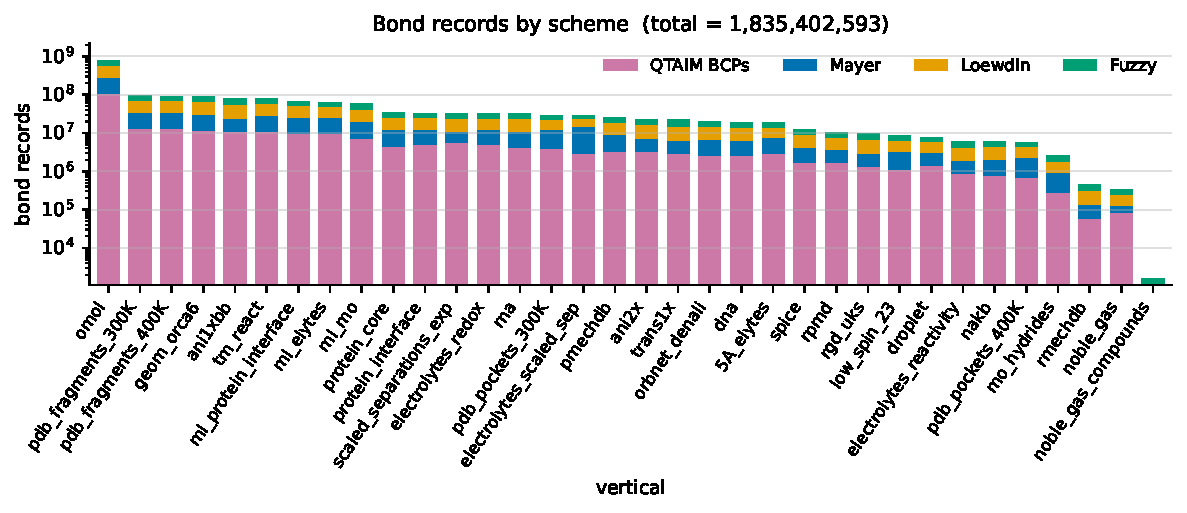
\includegraphics[width=\textwidth]{figures/census/bond_scheme_breakdown.pdf}
\caption{Per-vertical bond-order record counts, stacked by scheme
(QTAIM, Mayer, L\"owdin, fuzzy) on a log axis. Verticals are sorted by total
bond-record count. The four schemes report on the same set of bonds, so
counts represent records, not unique bond instances. Corpus total across
the four schemes is 1.83~billion records.}
\label{fig:bond_scheme_breakdown}
\end{figure}










 

 
\section{Evaluation Protocol}
\label{sec:eval}

% Keystone for the D\&B track. All counts anchored to the 2026-04-28 manifest
% (3,986,738 ok rows, 100\% read success).

\subsection{Tasks}
\label{sec:eval-tasks}

\begin{itemize}
  \item \textbf{T1 -- Per-atom partial charge regression.} Multi-target:
    \revised{ADCH, Becke, CM5, Hirshfeld, L\"owdin and Mulliken (six schemes)}
    jointly per atom. Headline:
    per-method, per-element MAE and Pearson $r$ on the test split.
  \item \textbf{T2 -- BCP property regression.} Targets: $\rho$,
    $\nabla^2\rho$, ellipticity at every QTAIM bond critical point.
    Headline: per-element-pair MAE on $\rho$, Pearson $r$ per pair,
    stratified by bond type (single, double, aromatic, metal-ligand)
    inferred from QTAIM topology.
  \item \textbf{T3 -- Bond classification.} Binary: does a QTAIM BCP
    exist between an atom pair within $2\times$ sum-of-covalent-radii.
    Compared against Mayer(Orca) / L\"owdin(ORCA) / fuzzy agreement. Headline: Macro-F1 plus
    per-element-pair confusion stats.
\end{itemize}

\subsection{Main Split}
\label{sec:eval-main-split}

The corpus is partitioned by molecular composition: \revised{each structure's
composition string -- the electronegativity-ordered formula produced by
\texttt{pymatgen}'s \texttt{Composition.formula} -- is hashed with SHA-256, mapped
to $[0,1)$, and assigned to train / val / test by cumulative thresholds
$0.8 / 0.1 / 0.1$. Because the key is an exact function of composition, every
structure sharing a composition receives the same assignment.}
Held-out sets (\S\ref{sec:eval-holdouts}) are excluded prior to \revised{hashing}, so no
structure appears as both an in-distribution test point and a stress-test point.
Hashing on composition rather than on row identity prevents near-duplicate
conformers of the same formula from crossing the train/val/test boundary.
\revised{Realized sizes are 3{,}125{,}019 / 398{,}982 / 403{,}951
(train / val / test) after excluding 58{,}786 held-out structures, which together
account for the full 3{,}986{,}738-structure corpus. Realized ratios are
79.6\,\% / 10.2\,\% / 10.3\,\% of the post-holdout corpus, within 0.4 percentage
points of the nominal targets.}
Verticals are not sampled uniformly because the split is global by formula; a
per-vertical post-split distribution table is provided in
\revised{App.~\ref{app:post_split}} as a transparency artifact.

\begingroup\color{revcolor}
\paragraph{Split leakage audit.}
Composition hashing removes exact-composition leakage but does not by itself
control scaffold- or homologue-level similarity, so we quantify both. No test
structure shares its exact composition with any training structure (0.0\,\%),
against 80.9\,\% for a row-level random split of the same corpus: same-composition
and conformer leakage are eliminated rather than reduced. Residual similarity is
real but bounded. Taking each test composition's nearest training neighbour among
compositions with an identical element set, 96.0\,\% of test compositions have such
a neighbour and it differs by a median of 5.3\,\% of the atom count. For
calibration, withholding the \texttt{tm\_react} vertical entirely raises that
median to 16.5\,\%, so the composition split sits roughly one third of the way from
a random split to a full vertical holdout. A direct homologue probe finds that
17.3\,\% of test compositions have a training composition differing by exactly one
CH$_2$ unit. We report these measurements rather than adding a Murcko scaffold
split because scaffold decomposition requires a sanitized covalent bond graph,
which is undefined for the transition-metal, ionic, multi-fragment and
reaction-path verticals that motivate this corpus: 27.0\,\% of structures contain
an element outside the organic subset that scaffold perception assumes, and
19.0\,\% contain a transition metal, lanthanide or actinide. A further observation
supports the stress-suite design in \S\ref{sec:eval-holdouts} over per-vertical
holdout: withholding \texttt{droplet} or \texttt{rna} entirely still leaves
67--68\,\% of their compositions matched exactly in training, because solvent
clusters and nucleotide fragments recur across verticals.
\endgroup

\subsection{Held-Out Evaluation Sets}
\label{sec:eval-holdouts}

Held-out sets are constructed independently of the main split. Membership is
decided from the manifest (and from \texttt{bond.lmdb} for the two metal-ligand
sets) and removed from train/val/test so no structure is evaluated as both
in-distribution test and stress-test. \revised{Where a set is subsampled
(H1, H3, H6), sampling is composition-stratified using a
BLAKE2b~\cite{10.1007/978-3-642-38980-1_8} rank over
\texttt{formula\_hill}, so the subsample is deterministic and reproducible.} Overlaps between held-out sets are allowed
(a structure can be both H7-large and H8-high-charge), but each set is generated
separately so error attributes to one axis. The headline signal per set is the
gap $\Delta = \mathrm{metric}_{\mathrm{held\text{-}out}} -
\mathrm{metric}_{\mathrm{main\,test}}$, reported alongside the absolute number;
a small $\Delta$ on H7 suggests size extrapolates, a large $\Delta$ on H1
indicates pair-level memorization. Three of the five sets (H1, H6, H7) inherit
the hardest axes from the OMol25 paper directly.

\paragraph{Sets and sizes.}
The five held-out sets together \revised{contain 60{,}578 records spanning 58{,}786
distinct structures} ($\sim$1.5\% of the dataset; \revised{overlaps allowed, and
1{,}792 records are structures belonging to two sets}):

\begin{itemize}
  \item \textbf{H1 -- Metal-ligand pairs (\revised{15{,}025}):} eleven (TM, partner) bond pairs sampled stratified across log-spaced frequency bands; selection driven by \emph{true} bonds (Mayer/fuzzy $\geq 0.3$) from \texttt{bond.lmdb}, not element co-occurrence (App.~\ref{app:heldout-h1}).
  \item \textbf{H3 -- Reactivity (\revised{12{,}506}):} composition-stratified subsample of \texttt{tm\_react} (5k), \texttt{electrolytes\_reactivity} (5k), \texttt{pmechdb} (2.5k); tests non-equilibrium and transition-state-adjacent geometries.
  \item \textbf{H6 -- Lanthanide-ligand pairs (2{,}589):} same construction as H1 applied to (Ln, partner) bonds (App.~\ref{app:heldout-h6}).
  \item \textbf{H7 -- Large systems (\revised{18{,}096}):} \texttt{n\_atoms > 250}; size extrapolation where fuzzy integration and grid-based QTAIM are most expensive and per-atom DFT SNR is hardest to maintain.
  \item \textbf{H8 -- Large net charges (\revised{12{,}362}):} \texttt{net\_charge\_abs > 4}; the high-charge tail where partial-charge schemes disagree most and SCF is most sensitive to functional and basis.
\end{itemize}

\revised{Counts are the records present in the released held-out LMDBs, verified
against each database's stored length. They fall a few records short of the
selection targets (H1 15{,}030, H3 12{,}507, H7 18{,}200, H8 12{,}393) where a
selected structure lacked a complete descriptor set at pull time.}

We deliberately use pair-level held-outs (H1, H6) rather than
whole-element held-outs because the goal of this benchmark is to produce
models that are usable across the periodic table. Holding out specific (metal, ligand) pairs keeps every element
represented in training while still measuring rare-chemistry transfer,
identical to OMol25.


\subsection{Methodology and Metrics}
\label{sec:eval-method}

All hyperparameter tuning and early stopping use the validation bucket; the test
bucket is reserved for a single final evaluation, with the same one-shot rule on
each held-out set. Metrics are MAE, RMSE, and Pearson $r$ per task. Stratifications:
\textbf{T1} per-method, per-element, per-vertical, per-charge-bucket; \textbf{T2}
per-element-pair, per-bond-type (covalent / metal-ligand / H-bond), per-vertical;
\textbf{T3} macro-F1 plus per-element-pair confusion.

\section{Limitations and Broader Impact}
\label{sec:limits}
% Level-of-theory transferability: functional inherited from OMol25.
% Not supported: force prediction, MD, conformational sampling.
% ECP artifacts, basis-set sensitivity.
% Rare chemistry counts with honest call-out.
% Open dataset and pipeline lower barrier to reproducible chemistry ML.
% Low dual-use risk.

This dataset is a subset of OMol25; release of the full electronic-structure
slice would scale us into the hundreds of billions of atom and bond records, but
we already cover the original's rich set of verticals. Descriptors are generated
exclusively with Multiwfn, so a cross-package benchmark against AIMAll~\citep{aimall}
or Critic2~\citep{critic2} would be a useful follow-up. Compute budget restricted
us to the Tier 0 features; future releases will add the more expensive schemes
relevant to other communities (MBIS for force-field~\citep{mbis} and MLIP
development~\citep{bamboo}, IBSI for bond-strength analysis~\citep{ibsi}).
\revised{The original work's energy and force labels are merged into the release
as \texttt{energy.lmdb}, aligned to the same per-structure keys across all
splits and held-out suites, enabling partial-charge-aware MLIP development.}

We are bound by the single level-of-theory used in OMol25 and so do not measure
descriptor sensitivity to basis set or functional. Prior work
by~\citet{D5DD00220F} found that QTAIM features can vary significantly across
LOTs while remaining useful for ML. OMol25 also covers only ground-state
calculations, so excited-state sensitivity is out of scope.

\textbf{Dual-use considerations.} The dual-use risk of this
release is minimal. The dataset surfaces interpretive electronic-structure
descriptors (charges, bond orders, QTAIM topology) on neutral and charged
molecules; it confers no obvious uplift for chemical, biological, or materials
threats beyond what the underlying OMol25 wavefunctions already permit. We
release the data and pipeline under an open license to support reproducibility
in chemistry ML.


\section{Conclusion}
\label{sec:conclusion}
% Three sentences. Recap claims. State dataset DOI.
We present OMol-Descriptors-4M: six partial charges, four bonding schemes, full
QTAIM topology, fuzzy descriptors, and ORCA globals across $\sim$4M structures
and 34 verticals, paired with a portable post-DFT pipeline and a held-out
evaluation protocol. This lowers the barrier for descriptor-aware surrogate
models across catalysis, drug discovery, and electrolyte design.

\section{Acknowledgments}
S.V. was supported by the DOE’s National Nuclear Security Administration’s Office of Defense Nuclear
Nonproliferation Research and Development (NA-22) as part of the NextGen Nonproliferation Leadership
Development Program. This work was also supported via grants from ALCF's Director Discretionary Allocations 
and compute on LLNL's center provided via NA-22.  

\bibliography{bib/refs}
\bibliographystyle{plainnat}

\begin{hide}
\section*{Acknowledgments}
S.V. is supported by the NextGen program. NextGen is supported by the National Nuclear Security Administration's (NNSA)
Office of Defense Nuclear Nonproliferation Research and Development (NA-22)
through the Nonproliferation Stewardship Program (NSP).
Computing resources were provided by the Tuolumne system at Lawrence Livermore
National Laboratory, the Argonne
Leadership Computing Facility, and the Lawrencium high-performance
computing cluster at Lawrence Berkeley National Laboratory.
We thank the OMol25 team for releasing the underlying wavefunctions, density
matrices, and ORCA outputs that make this work possible.
\end{hide}
\newpage

\input{checklist}

\newpage
\appendix
\section{Datasheet for Datasets}
\label{app:datasheet}

\paragraph{Motivation.}
OMol-Descriptors-4M was created to extend the OMol25 corpus~\citep{levine2026openmolecules2025omol25} with
post-DFT interpretive descriptors: partial charges, bond orders, QTAIM
topology, fuzzy and surface integrations, and ORCA global features (which where in OMol25) that have
historically been absent from large-scale ML-ready quantum-chemical datasets.
The dataset is intended for training descriptor-aware ML models and for
benchmarking surrogates that approximate wavefunction-derived quantities
without per-molecule DFT.
The dataset was created by the authors at the authors' home institution.
Funding sources are listed in the Acknowledgments.

\paragraph{Composition.}
Each instance is a single molecular structure with associated wavefunction-derived
descriptors. The corpus contains 3{,}986{,}738 structures (the publicly released
4M wavefunction subset of OMol25) spanning 80+
elements. Per-structure data is sharded across eight LMDB files
(Section~\ref{sec:storage}); the descriptor families are enumerated in
Section~\ref{sec:dataset}. Splits are described in Section~\ref{sec:eval}.
The corpus contains no human subjects, personally identifiable information, or
confidential data.

\paragraph{Collection Process.}
Geometries, wavefunctions, density matrices, and ORCA output files were
inherited from the OMol25 4M electronic structure release. We did not collect new DFT calculations;
all post-processing was applied to artifacts already produced by the OMol25
authors at the $\omega$B97M-V/def2-TZVPD level.

\paragraph{Preprocessing / Cleaning / Labeling.}
Wavefunctions were processed through the open \texttt{generator} pipeline
(Section~\ref{sec:pipeline}), wrapping Multiwfn~\citep{multiwfn} and
ORCA~\citep{orca5} post-analysis utilities. JSON outputs were validated and
compacted into LMDB shards keyed by relative job-folder path. Conversion is
essentially lossless (Section~\ref{sec:dataset-quality}); all raw artifacts
remain available in the OMol25 release for users wishing to reprocess.

\paragraph{Uses.}
Intended uses include training ML models that predict charges, bond orders,
or QTAIM properties; benchmarking descriptor-aware MLIPs; and serving as a
target for surrogate models that compress the full DFT-then-Multiwfn pipeline.
Inappropriate uses include drawing chemistry conclusions outside the OMol25
level of theory or extrapolating to excited-state regimes (see \S\ref{sec:limits}).

\paragraph{Distribution.}
The dataset is released on Hugging Face under a CC-BY-4.0 license, inheriting
OMol25's license terms: \url{https://huggingface.co/datasets/neuripssub2026test/OMol-Descriptors-4M}.
The \texttt{generator} pipeline is released under MIT license at
\url{https://anonymous.4open.science/r/qtaim_generator-8C0C/README.md}. No third-party IP, export controls, or fees
apply.

\paragraph{Maintenance.}
The dataset will be maintained by the authors at Lawrence Berkeley National
Laboratory. Issues, errata, and feature requests can be filed on the code
repository. Updates, including the planned merge with OMol25 energies and
forces, and additional descriptor schemes (MBIS, IBSI, CHELPG), will be
released as versioned HF records with changelogs. Older versions will
remain accessible.

\section{Compute Resources}
\label{app:compute}

Post-processing of the 4M-structure subset was carried out on
three HPC systems:

\begin{itemize}
  \item \textbf{Tuolumne} (Lawrence Livermore National Laboratory). El Capitan
    sibling system used for the highest-throughput phase of Multiwfn-driven
    QTAIM, charge, bond-order, and fuzzy-integration jobs.
    \url{https://hpc.llnl.gov/hardware/compute-platforms/tuolumne}
  \item \textbf{ALCF Crux} (Argonne Leadership Computing Facility, Argonne
    National Laboratory). AMD EPYC-based system used for additional
    descriptor generation and Parsl-managed workflow batches.
    \url{https://www.alcf.anl.gov/crux}
  \item \textbf{Lawrencium LR7, LR6 partitions} (Lawrence Berkeley National
    Laboratory High-Performance Computing). Used for ORCA conversions
    (\texttt{orca\_2mkl}), JSON-to-LMDB sharded conversion, and analytical
    notebook workloads.
    \url{https://scienceit-docs.lbl.gov/hpc/systems/lawrencium/}
\end{itemize}


\section{Held-Out Construction Logic}
\label{app:heldout}
% Detailed construction for H1--H8.

\subsection{H1 metal-ligand pair selection}
\label{app:heldout-h1}

\begin{itemize}
  \item Element-pair co-occurrence (859 TM pairs in
    \texttt{metal\_nonmetal\_pairs.csv}) is a coarse upper bound;
    selection here uses true bonds (Mayer / fuzzy bond order $\geq 0.3$)
    extracted from \texttt{bond.lmdb} via \texttt{tm\_neighbor\_lists.py}.
  \item Per-vertical bond extraction across 15 TM-bearing verticals;
    one row per (TM atom, partner atom) bond.
  \item Global pair table: \textbf{1{,}101 unique (TM, partner) bond
    pairs} across \textbf{651{,}742 TM-bonded structures} (16.35\% of
    dataset).
  \item Frequency bands (log-spaced): B1 $[1,10)$ 529 pairs;
    B2 $[10,100)$ 93; B3 $[100,1k)$ 233; B4 $[1k,10k)$ 203;
    B5 $[10k,100k)$ 43.
  \item Stratified sampling shape $(3, 2, 2, 4, 0)$,
    \texttt{numpy.random.default\_rng(seed=87)}. B5 excluded (Pt-C,
    Ti-H, etc. dominate training); B4 capped at 4 to keep realized
    holdout near 15k.
  \item Selected pairs: \emph{B1} Pt-Na, Rh-Fe, Ag-Pd; \emph{B2} Sc-Ir,
    Cd-Sb; \emph{B3} Mn-Sb, Ir-Ge; \emph{B4} Tc-Cl, Re-H, Sc-S, Hf-C.
  \item Variance: across 30 seeds with shape $(3,2,2,4,0)$, realized
    size is $15{,}227 \pm 4{,}871$. Seed 87 lands within 200 of the 15k
    target.
  \item Reproducibility:
    \texttt{qtaim\_gen/source/analysis/build\_holdout\_csvs.py}; outputs
    \texttt{h1\_metal\_ligand\_pair\_definitions.csv} and
    \texttt{h1\_metal\_ligand\_pairs.csv}.
\end{itemize}

\subsection{H6 lanthanide-ligand pair selection}
\label{app:heldout-h6}

\begin{itemize}
  \item Same construction as H1, applied to (Ln, partner) bonds via
    \texttt{tm\_neighbor\_lists.py --element\_class ln}.
  \item Five Ln-bearing verticals: \texttt{omol}, \texttt{tm\_react},
    \texttt{ml\_mo}, \texttt{electrolytes\_reactivity},
    \texttt{mo\_hydrides}.
  \item Global pair table: \textbf{453 unique (Ln, partner) bond pairs}
    across \textbf{66{,}677 Ln-bonded structures} (1.67\% of dataset).
    All 15 lanthanides represented.
  \item Frequency bands: B1=207, B2=102, B3=86, B4=58, B5=0 (max pair
    size 4{,}439). H6 effectively samples four bands.
  \item Stratified sampling shape $(3, 2, 2, 1, 0)$, \texttt{seed=190}.
    B4 toned down to 1 vs H1's 4 (Ln B4 is sparser, target $\sim$2.5k).
  \item Selected pairs: \emph{B1} Lu-Ni, Ce-La, Gd-Sb; \emph{B2} Ho-F,
    Yb-Si; \emph{B3} Dy-S, Nd-S; \emph{B4} Tm-N.
  \item Reproducibility: same build script as H1; outputs
    \texttt{h6\_lanthanide\_ligand\_pair\_definitions.csv} and
    \texttt{h6\_lanthanide\_ligand\_pairs.csv}.
\end{itemize}

\subsection{Holdout-Aware Splitting Pipeline}
\label{sec:eval-pipeline}

\begin{itemize}
  \item \textbf{Step 1 -- Pull holdouts.}
    \texttt{pull\_holdout\_records.py} reads each holdout CSV,
    materializes per-set LMDBs under \texttt{data/holdouts/<set>/}, and
    emits a \texttt{manifest\_holdout.parquet} keyed on the LMDB key
    convention
    \texttt{relpath(folder, root\_dir).replace(os.sep, "\_\_")}.
  \item \textbf{Step 2 -- Exclude.}
    \texttt{multi\_vertical.load\_exclusion\_set} re-derives LMDB keys
    from the manifest \texttt{rel\_path} column and unions
    H1/H3/H6/H7/H8 into one per-vertical exclusion set.
  \item \textbf{Step 3 -- Split.} \texttt{split\_descriptor\_lmdbs.py}
    reads \texttt{structure.lmdb}, drops excluded keys, assigns each
    remaining key to train/val/test by
    \texttt{BLAKE2b(formula\_hill) \% 10}, then partitions each of the
    8 descriptor LMDBs (\texttt{structure}, \texttt{charge},
    \texttt{qtaim}, \texttt{bond}, \texttt{fuzzy}, \texttt{other},
    \texttt{orca}, \texttt{timings}) into the assigned split.
  \item Output layout:
    \texttt{<output\_dir>/<vertical>/<split>/<descriptor>.lmdb}.
  \item HPC parallelism: \texttt{--include\_verticals X} +
    \texttt{--merge\_from DIR}, mirroring the pull pipeline.
    Per-vertical \texttt{split\_assignment.json} is the durable,
    race-free record (no global plan file).
  \item Lock-step audit: across all 8 descriptors, source row count $=$
    train $+$ val $+$ test $+$ excluded for every vertical (verified on
    \texttt{ani2x}: 215{,}642 source $=$ 168{,}783 + 17{,}417 +
    29{,}442, $n_{\mathrm{excluded}}=0$).
\end{itemize}

%\section{Per-Method Descriptor Definitions}
%\label{app:descriptors}

%\section{HPC Configuration Files}
%\label{app:hpc}
% NERSC + ALCF Parsl configs.

\section{Per-Vertical Census Table}
\label{app:t1_census}

Table~\ref{tab:t1_census} expands Sec.~\ref{sec:census} into the full
per-vertical breakdown (34 verticals plus the corpus total).
Figure~\ref{fig:descriptor_density_app} reports per-structure descriptor
density for atoms and QTAIM bond critical points.

\begin{scriptsize}
\setlength{\tabcolsep}{2.5pt}
\begin{longtable}{lrrrrrrrr}
\caption{Per-vertical census of OMol-Descriptors-4M. Counts are
corpus-level pre-split totals. \textit{Structs}: structure count.
\textit{Forms}: unique alphabetical formulas. \textit{Atoms}: atom-level
descriptor records. \textit{Charge rec.}: per-job per-method charge-scheme
records. \textit{BCPs}: QTAIM bond critical points.
\textit{Mayer / L\"owdin / Fuzzy}: per-scheme bond-order records.}
\label{tab:t1_census} \\
\toprule
Vertical & Structs & Forms & Atoms & Charge rec. & BCPs & Mayer & L\"owdin & Fuzzy \\
\midrule
\endfirsthead
\multicolumn{9}{l}{\small\textit{Table~\ref{tab:t1_census} continued from previous page}} \\
\toprule
Vertical & Structs & Forms & Atoms & Charge rec. & BCPs & Mayer & L\"owdin & Fuzzy \\
\midrule
\endhead
\midrule
\multicolumn{9}{r}{\small\textit{continued on next page}} \\
\endfoot
\bottomrule
\endlastfoot
\texttt{5A\_elytes}              &     14{,}200 &     11{,}294 &   2{,}325{,}187 &      99{,}383 &   2{,}982{,}866 &    4{,}474{,}371 &    6{,}655{,}293 &    4{,}244{,}442 \\
\texttt{ani1xbb}                 &    737{,}208 &     48{,}320 &  10{,}834{,}251 &   7{,}318{,}728 &  10{,}801{,}957 &   12{,}465{,}497 &   30{,}634{,}609 &   28{,}118{,}840 \\
\texttt{ani2x}                   &    215{,}642 &      5{,}773 &   3{,}280{,}277 &   1{,}586{,}066 &   3{,}346{,}555 &    3{,}824{,}490 &    9{,}516{,}073 &    6{,}379{,}670 \\
\texttt{dna}                     &     24{,}647 &      4{,}312 &   2{,}186{,}892 &     172{,}529 &   2{,}559{,}225 &    3{,}843{,}725 &    7{,}372{,}380 &    4{,}907{,}003 \\
\texttt{droplet}                 &     18{,}694 &      3{,}376 &   1{,}109{,}505 &     130{,}858 &   1{,}457{,}592 &    1{,}653{,}393 &    2{,}805{,}247 &    1{,}785{,}875 \\
\texttt{electrolytes\_reactivity} &     66{,}967 &     18{,}063 &     874{,}449 &     468{,}769 &     887{,}548 &      986{,}445 &    2{,}340{,}553 &    1{,}953{,}147 \\
\texttt{electrolytes\_redox}      &     46{,}069 &     33{,}579 &   4{,}017{,}583 &     322{,}483 &   4{,}945{,}260 &    7{,}442{,}261 &   11{,}512{,}752 &    9{,}064{,}929 \\
\texttt{electrolytes\_scaled\_sep}&     30{,}768 &     21{,}186 &   2{,}307{,}396 &     215{,}369 &   2{,}847{,}853 &   11{,}683{,}800 &    8{,}801{,}619 &    5{,}116{,}940 \\
\texttt{geom\_orca6}              &    199{,}805 &     36{,}054 &  10{,}321{,}888 &   1{,}398{,}634 &  11{,}579{,}867 &   18{,}310{,}972 &   35{,}343{,}998 &   22{,}839{,}614 \\
\texttt{low\_spin\_23}             &     12{,}939 &     12{,}045 &     927{,}730 &      90{,}573 &   1{,}113{,}772 &    2{,}194{,}086 &    3{,}228{,}506 &    2{,}213{,}493 \\
\texttt{ml\_elytes}               &     51{,}560 &     35{,}054 &   7{,}608{,}642 &     360{,}904 &   9{,}672{,}793 &   15{,}638{,}665 &   22{,}494{,}066 &   13{,}464{,}794 \\
\texttt{ml\_mo}                   &     77{,}603 &     40{,}658 &   6{,}098{,}677 &     543{,}153 &   7{,}336{,}479 &   12{,}931{,}862 &   20{,}795{,}278 &   17{,}937{,}539 \\
\texttt{ml\_protein\_interface}    &     61{,}856 &     35{,}118 &   8{,}314{,}895 &     432{,}979 &   9{,}480{,}078 &   16{,}584{,}221 &   26{,}101{,}394 &   15{,}494{,}518 \\
\texttt{mo\_hydrides}             &      3{,}396 &      2{,}870 &     232{,}942 &      23{,}772 &     280{,}311 &      664{,}784 &      851{,}813 &      781{,}762 \\
\texttt{nakb}                    &      5{,}606 &      1{,}188 &     651{,}552 &      50{,}642 &     777{,}349 &    1{,}297{,}268 &    2{,}280{,}331 &    1{,}551{,}414 \\
\texttt{noble\_gas}               &      1{,}915 &        136 &      66{,}993 &      13{,}651 &      84{,}800 &       43{,}394 &      116{,}497 &       87{,}580 \\
\texttt{noble\_gas\_compounds}     &         18 &         12 &         189 &         126 &         179 &          326 &          560 &          518 \\
\texttt{omol}                    &  1{,}428{,}279 &    593{,}876 &  92{,}071{,}794 &   9{,}997{,}947 & 109{,}334{,}787 &  170{,}492{,}089 &  291{,}413{,}475 &  218{,}967{,}571 \\
\texttt{orbnet\_denali}           &     51{,}102 &     30{,}339 &   2{,}305{,}764 &     357{,}714 &   2{,}594{,}095 &    4{,}028{,}552 &    7{,}875{,}696 &    5{,}188{,}774 \\
\texttt{pdb\_fragments\_300K}      &     93{,}334 &     68{,}881 &  11{,}255{,}165 &     653{,}329 &  13{,}208{,}426 &   21{,}291{,}730 &   36{,}314{,}068 &   22{,}292{,}731 \\
\texttt{pdb\_fragments\_400K}      &     92{,}698 &     68{,}485 &  11{,}177{,}181 &     648{,}881 &  13{,}058{,}825 &   20{,}774{,}760 &   36{,}149{,}798 &   22{,}215{,}370 \\
\texttt{pdb\_pockets\_300K}        &     16{,}870 &     15{,}453 &   3{,}245{,}155 &     118{,}069 &   3{,}915{,}033 &    8{,}616{,}479 &   10{,}415{,}619 &    6{,}407{,}044 \\
\texttt{pdb\_pockets\_400K}        &      3{,}204 &      3{,}092 &     630{,}613 &      22{,}422 &     701{,}104 &    1{,}658{,}125 &    2{,}019{,}313 &    1{,}222{,}919 \\
\texttt{pmechdb}                 &     49{,}832 &     28{,}171 &   2{,}951{,}782 &     379{,}418 &   3{,}316{,}002 &    6{,}028{,}189 &    9{,}928{,}066 &    6{,}572{,}474 \\
\texttt{protein\_core}            &     35{,}406 &     14{,}980 &   4{,}197{,}118 &     247{,}840 &   4{,}436{,}976 &    8{,}229{,}618 &   13{,}219{,}684 &    7{,}738{,}794 \\
\texttt{protein\_interface}       &     44{,}760 &     16{,}127 &   4{,}298{,}048 &     313{,}320 &   4{,}938{,}560 &    7{,}052{,}373 &   13{,}235{,}662 &    8{,}007{,}220 \\
\texttt{rgd\_uks}                 &     75{,}316 &        980 &   1{,}337{,}124 &     527{,}212 &   1{,}340{,}336 &    1{,}504{,}737 &    3{,}810{,}675 &    3{,}314{,}638 \\
\texttt{rmechdb}                 &      2{,}803 &        731 &      58{,}528 &      28{,}024 &      59{,}403 &       76{,}928 &      171{,}675 &      150{,}328 \\
\texttt{rna}                     &     34{,}434 &      5{,}168 &   3{,}661{,}659 &     241{,}036 &   4{,}108{,}650 &    7{,}166{,}774 &   12{,}646{,}859 &    8{,}583{,}065 \\
\texttt{rpmd}                    &     18{,}652 &      2{,}992 &   1{,}412{,}713 &     152{,}365 &   1{,}721{,}533 &    2{,}025{,}287 &    3{,}893{,}696 &    2{,}478{,}985 \\
\texttt{scaled\_separations\_exp} &     53{,}180 &     37{,}168 &   5{,}020{,}630 &     372{,}260 &   5{,}549{,}452 &    5{,}214{,}145 &   13{,}616{,}510 &    8{,}822{,}261 \\
\texttt{spice}                   &     44{,}447 &     19{,}603 &   1{,}553{,}948 &     311{,}129 &   1{,}686{,}049 &    2{,}413{,}029 &    4{,}992{,}500 &    3{,}292{,}358 \\
\texttt{tm\_react}                &    158{,}189 &     86{,}819 &   9{,}209{,}119 &   1{,}107{,}323 &  10{,}873{,}610 &   17{,}179{,}722 &   29{,}890{,}848 &   22{,}389{,}065 \\
\texttt{trans1x}                 &    213{,}731 &        171 &   2{,}974{,}386 &   1{,}496{,}117 &   2{,}977{,}381 &    3{,}345{,}716 &    8{,}459{,}481 &    7{,}799{,}805 \\
\midrule
\textbf{TOTAL}                   &  3{,}985{,}130 &  1{,}302{,}074 & 218{,}519{,}775 &  30{,}203{,}025 & 253{,}974{,}706 &  401{,}137{,}813 &  688{,}904{,}594 &  491{,}385{,}480 \\
\end{longtable}
\end{scriptsize}

\begin{figure}[h]
\centering
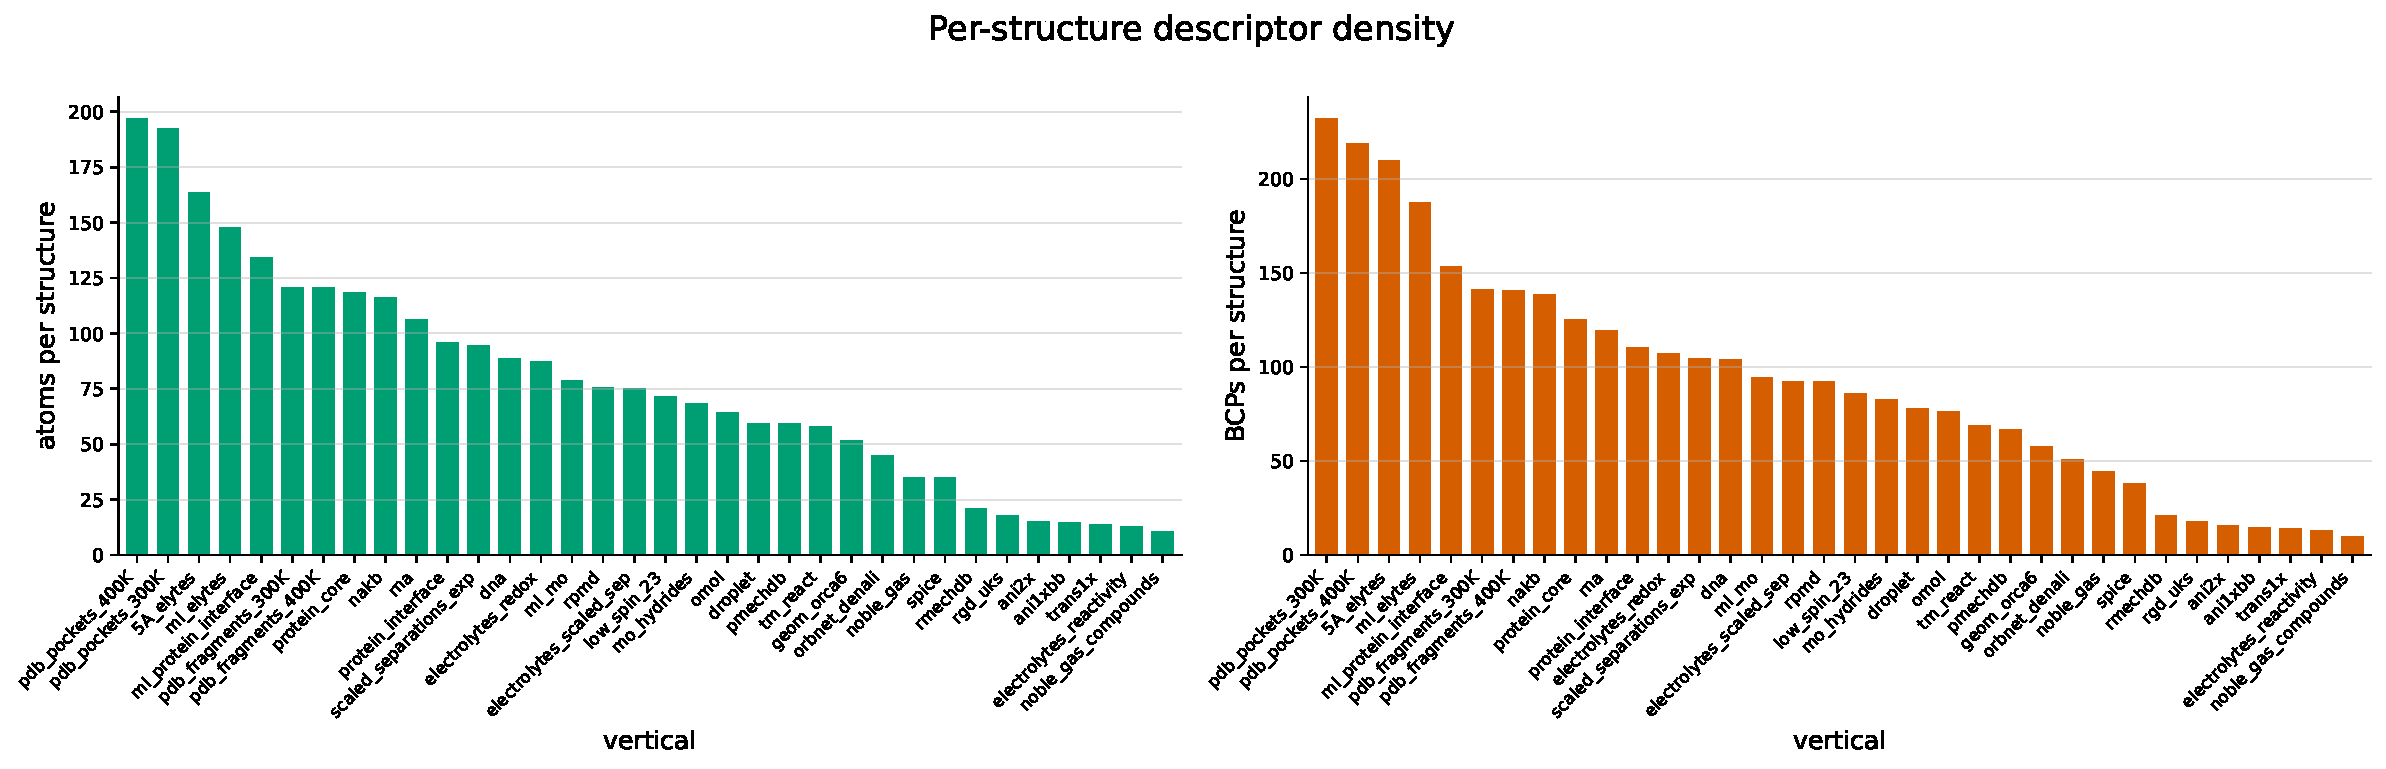
\includegraphics[width=\textwidth]{figures/census/descriptor_density.pdf}
\caption{Per-structure descriptor density across the 34 verticals.
Left: atoms per structure. Right: QTAIM bond critical points per
structure. Solvated-protein verticals (\texttt{pdb\_pockets\_300K},
\texttt{pdb\_pockets\_400K}, \texttt{protein\_core}) form the high-density
tail; \texttt{noble\_gas\_compounds} sits at the low end as the sparse
limit.}
\label{fig:descriptor_density_app}
\end{figure}

\begin{figure}[h]
\centering
\includegraphics[width=\textwidth]{figures/census/bond_scheme_breakdown_grouped.png}
\caption{Per-vertical bond-record counts shown as grouped bars rather than
stacked. The log-scale stack in Fig.~\ref{fig:bond_scheme_breakdown} compresses
the non-QTAIM schemes against the QTAIM BCP totals; the grouped view confirms
that Mayer, L\"owdin, and fuzzy bond records are within roughly an order of
magnitude of QTAIM BCP counts on every vertical, i.e. the four schemes have
comparable coverage rather than QTAIM dominating.}
\label{fig:bond_scheme_grouped_app}
\end{figure}


\subsection{Sharded Execution and LMDB Merge}
% Figure F4: sharding schematic.

LMDB is single-writer and exhibits lock contention under naive parallel writes, so
\texttt{json-to-lmdb} does not attempt to share a single output environment across workers.
Instead, each parallel job is given a shard index $i \in \{0, \dots, N-1\}$ and a total shard
count $N$, and partitions the input folder list by index modulo $N$. For the flat
\textit{root/category/subset/job} hierarchy this is a glob plus a modulo filter; for jagged
hierarchies such as OMol4M, where job folders sit at variable depth, the user supplies an
explicit \texttt{--folder\_list} file of absolute paths and the same modulo partitioning
applies to the line index. In both cases the LMDB key is
\texttt{relpath(folder, root\_dir).replace(os.sep, "\_\_")}, which is identical across every
descriptor family, so the per-family shards always share keys and joining is trivial.

Each shard writes into its own subdirectory as \texttt{shard\_\{i\}.lmdb}. When the last
shard finishes its work it drops a sentinel file (\texttt{shard\_N.done}); the merge step
waits on the full sentinel set and then concatenates per-family shards into a single
consolidated LMDB per family. The same shard/merge pattern is implemented at the converter
stage in \texttt{converter.py}, so graph construction can also be parallelized and joined
into one final per-vertical graph LMDB.


\section{LMDB Conversion Quality Audit}
\label{app:lmdb_audit}

Table~\ref{tab:lmdb_quality} reports raw failure counts per vertical from the
post-conversion audit (\texttt{lmdb\_status\_audit.py}).
\textit{QTAIM fail}: records where the \texttt{qtaim.lmdb} entry is empty,
malformed, or unpickleable.
\textit{ORCA fail}: same for \texttt{orca.lmdb} (includes SCF non-convergence
flagged at the parse stage).
\textit{Other fail}: failures across \texttt{structure}, \texttt{charge},
\texttt{bond}, \texttt{fuzzy}, and \texttt{other} LMDBs (all zero in this
release).
\textit{Max drop}: largest number of \texttt{structure.lmdb} keys absent from
any single descriptor LMDB; values $\leq 4$ across all verticals.

\begin{table}[h]
\centering
\caption{Per-vertical LMDB conversion-quality audit. Verticals with all
zeros across the four failure columns are shown as ``--''.}
\label{tab:lmdb_quality}
\begin{tabular}{lrrrrr}
\toprule
Vertical & $N$ & QTAIM fail & ORCA fail & Other fail & Max drop \\
\midrule
  \texttt{omol} & 1,429,192 & 17 & 896 & 0 & 1 \\
  \texttt{ani1xbb\_reparse} & 737,210 & 2 & 0 & 0 & 0 \\
  \texttt{ani2x} & 215,642 & -- & -- & -- & -- \\
  \texttt{trans1x} & 213,731 & -- & -- & -- & -- \\
  \texttt{geom\_orca6} & 199,805 & -- & -- & -- & -- \\
  \texttt{tm\_react} & 158,190 & 0 & 1 & 0 & 0 \\
  \texttt{pdb\_fragments\_300K} & 93,334 & 0 & 0 & 0 & 1 \\
  \texttt{pdb\_fragments\_400K} & 92,698 & -- & -- & -- & -- \\
  \texttt{ml\_mo} & 77,603 & 1 & 23 & 0 & 0 \\
  \texttt{rgd\_uks} & 75,316 & -- & -- & -- & -- \\
  \texttt{electrolytes\_reactivity} & 66,974 & 0 & 7 & 0 & 0 \\
  \texttt{ml\_protein\_interface} & 61,859 & 0 & 3 & 0 & 0 \\
  \texttt{scaled\_separations\_exp} & 53,219 & 2 & 37 & 0 & 0 \\
  \texttt{ml\_elytes} & 51,599 & 1 & 38 & 0 & 0 \\
  \texttt{orbnet\_denali} & 51,102 & -- & -- & -- & -- \\
  \texttt{pmechdb} & 49,832 & -- & -- & -- & -- \\
  \texttt{electrolytes\_redox} & 46,081 & 0 & 12 & 0 & 0 \\
  \texttt{protein\_interface} & 44,972 & 0 & 212 & 0 & 0 \\
  \texttt{spice} & 44,450 & 1 & 2 & 0 & 4 \\
  \texttt{protein\_core} & 35,406 & -- & -- & -- & -- \\
  \texttt{rna} & 34,745 & 0 & 311 & 0 & 0 \\
  \texttt{electrolytes\_scaled\_sep} & 30,769 & 0 & 1 & 0 & 0 \\
  \texttt{dna} & 24,647 & -- & -- & -- & -- \\
  \texttt{droplet} & 18,694 & -- & -- & -- & -- \\
  \texttt{rpmd} & 18,652 & 0 & 0 & 0 & 1 \\
  \texttt{pdb\_pockets\_300K} & 16,927 & 0 & 57 & 0 & 0 \\
  \texttt{5A\_elytes} & 14,202 & 0 & 2 & 0 & 2 \\
  \texttt{low\_spin\_23} & 12,939 & -- & -- & -- & -- \\
  \texttt{nakb} & 5,606 & -- & -- & -- & -- \\
  \texttt{mo\_hydrides} & 3,396 & -- & -- & -- & -- \\
  \texttt{pdb\_pockets\_400K} & 3,210 & 1 & 5 & 0 & 0 \\
  \texttt{rmechdb} & 2,803 & -- & -- & -- & -- \\
  \texttt{noble\_gas} & 1,915 & -- & -- & -- & -- \\
  \texttt{noble\_gas\_compounds} & 18 & -- & -- & -- & -- \\
\midrule
  \textbf{Total} & 3,986,738 & 25 & 1607 & 0 & 4 \\
\bottomrule
\end{tabular}
\end{table}

\vspace{1em}
Figure~\ref{fig:descriptor_coverage} shows per-method descriptor coverage
across all 34 verticals. Rows are descriptor methods grouped by family;
columns are verticals ordered by structure count (largest left).
Universal methods (Hirshfeld, ADCH, CM5, Becke charges; Fuzzy bond orders;
ORCA Mayer/L\"owdin/SCF/gradient/dipole) reach $\geq$99\% on every vertical.
QTAIM critical-point records achieve $\geq$99.9\% coverage.

\begin{figure}[h]
\centering
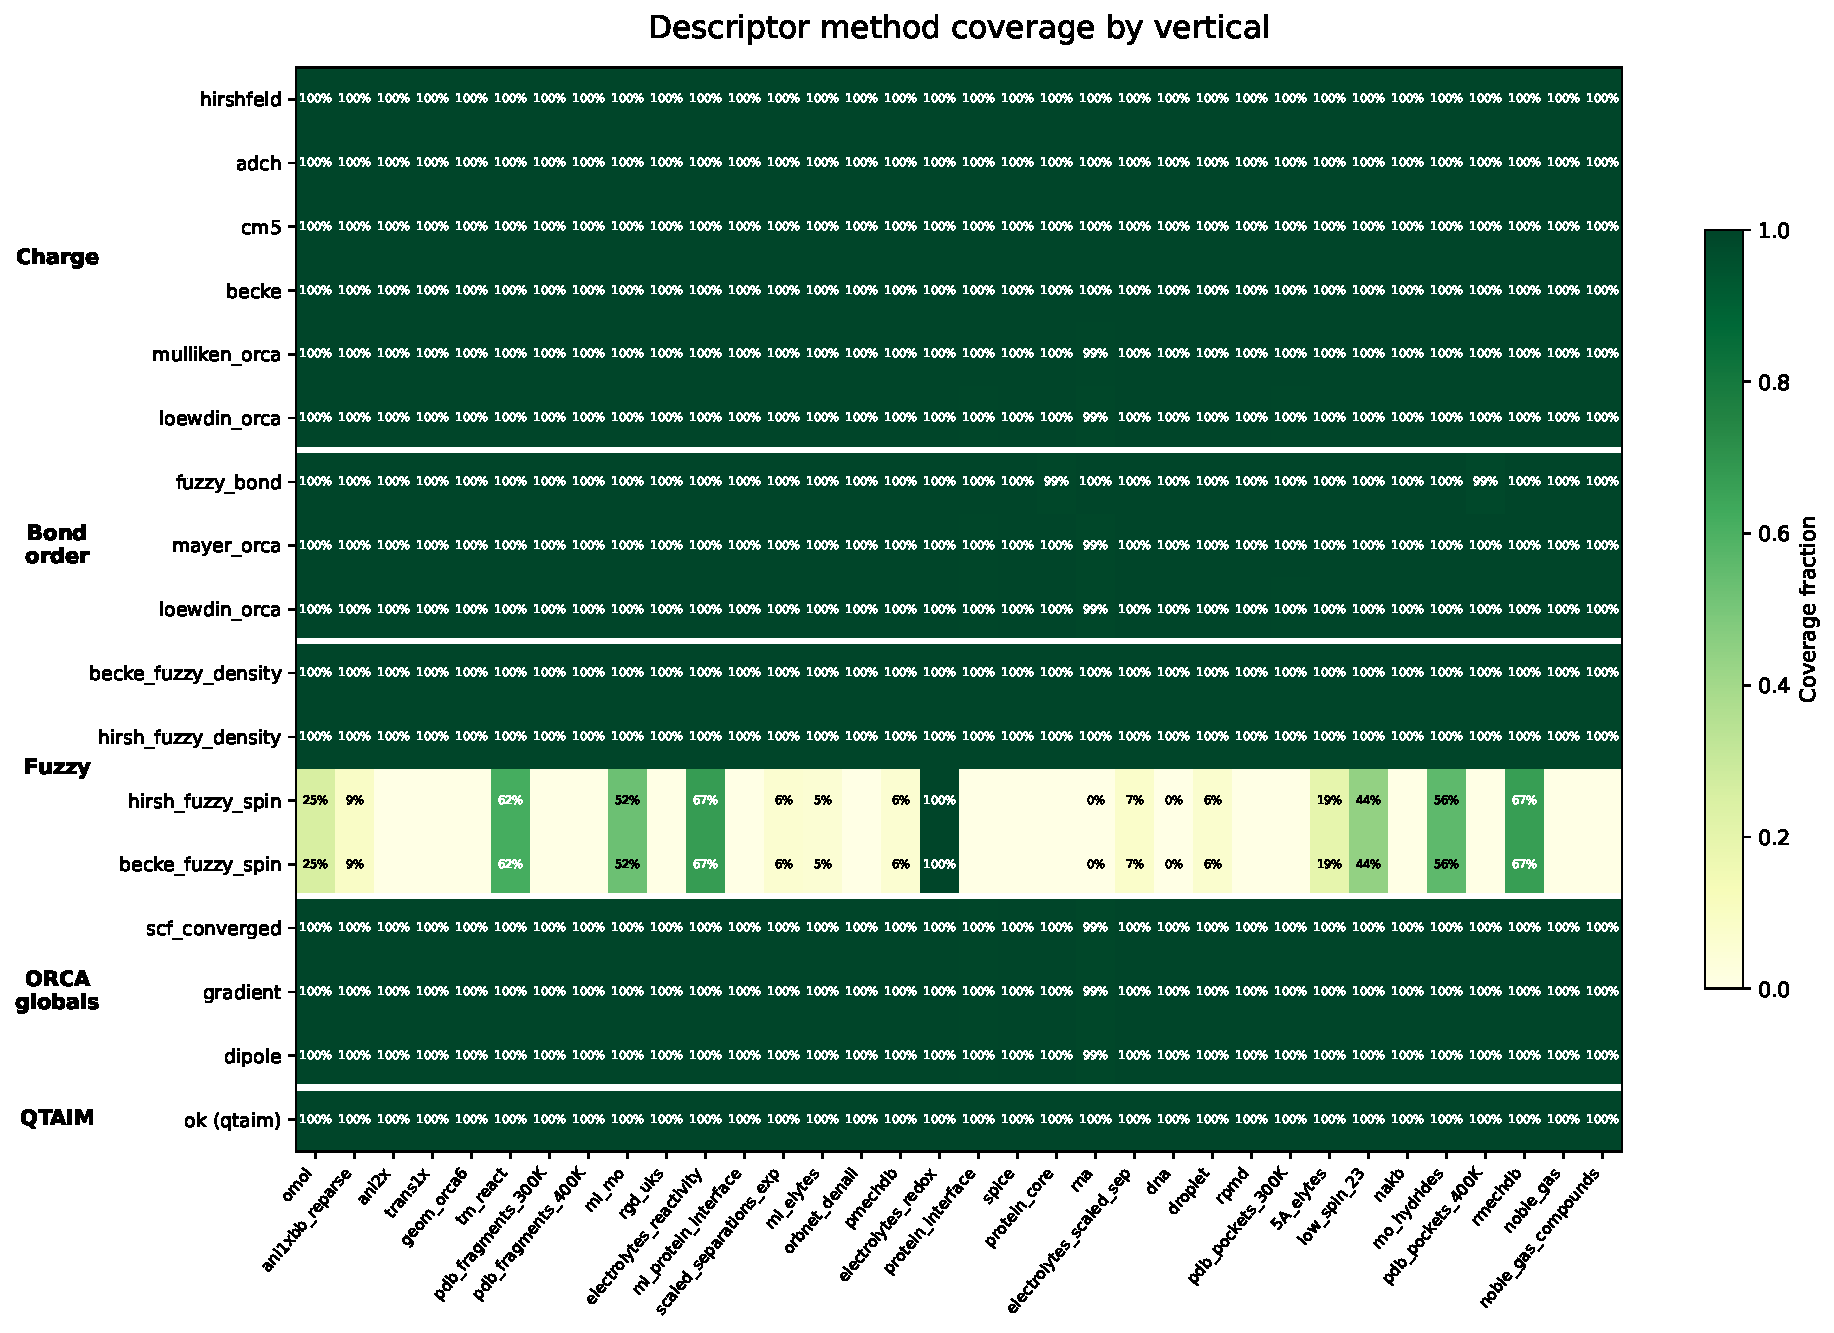
\includegraphics[width=\textwidth]{figures/dataset/dataset_coverage_heatmap.pdf}
\caption{Per-method descriptor coverage fraction across all 34 verticals.
Green = full coverage; white = absent. Vertical white lines separate
descriptor families. The single \texttt{ok (qtaim)} column reports
$\texttt{qtaim.lmdb}$ record validity.}
\label{fig:descriptor_coverage}
\end{figure}


\section{Charge-Scheme Cross-Correlations}
\label{app:charge_correlations}

We quantify pairwise agreement across the six partial-charge schemes
(Hirshfeld, CM5, ADCH, Becke, Mulliken, L\"{o}wdin) using two symmetric
metrics computed over all atom-level charge records in the corpus:
pairwise $R^2$ (coefficient of determination between scheme $a$ and scheme $b$
over all atoms) and mean absolute error (MAE, in electron units).
Figures~\ref{fig:charge_pearson_overall} and~\ref{fig:charge_mae_overall}
show the corpus-wide matrices; Figures~\ref{fig:charge_pearson_per_element_class}
and~\ref{fig:charge_pearson_tm} break these down by element class and by individual
transition metal; Figure~\ref{fig:charge_pearson_per_vertical} shows per-vertical matrices.

\begin{figure}[h]
\centering
\includegraphics[width=0.55\textwidth]{figures/charge/corpus_charge_pearson_overall.png}
\caption{Corpus-wide pairwise $R^2$ between charge schemes over all $\sim$218M atom
records. Hirshfeld--CM5 ($R^2=0.77$) and Hirshfeld--ADCH ($R^2=0.53$) show the
strongest cross-scheme agreement; Mulliken and L\"{o}wdin correlate weakly with
the stockholder-partitioned schemes ($R^2 \leq 0.30$).}
\label{fig:charge_pearson_overall}
\end{figure}

\begin{figure}[h]
\centering
\includegraphics[width=0.55\textwidth]{figures/charge/corpus_charge_mae.png}
\caption{Corpus-wide pairwise MAE (in $e$) between charge schemes.
Hirshfeld--CM5 (0.093~$e$) and Hirshfeld--ADCH (0.113~$e$) have the smallest
cross-scheme deviation. Mulliken diverges most ($\geq$0.37~$e$ versus
Hirshfeld/CM5/ADCH; 0.469~$e$ versus L\"{o}wdin), consistent with its
basis-set sensitivity at the def2-TZVPD level used throughout OMol25.}
\label{fig:charge_mae_overall}
\end{figure}

\begin{figure}[h]
\centering
\includegraphics[width=0.9\textwidth]{figures/charge/corpus_charge_pearson_per_element.png}
\caption{Pairwise $R^2$ stratified by element class: main-group, transition-metal,
lanthanide, and noble-gas subsets. Inter-scheme agreement tracks the corpus-wide
pattern within main-group chemistry; transition metals and lanthanides show reduced
Hirshfeld--ADCH agreement, reflecting the influence of $d$/$f$ polarization on
atomic-basin integration.}
\label{fig:charge_pearson_per_element_class}
\end{figure}

\begin{figure}[h]
\centering
\includegraphics[width=0.85\textwidth]{figures/charge/corpus_charge_pearson_transition_metals.png}
\caption{Pairwise $R^2$ broken down by individual transition-metal element
(30 panels, $n$ = atoms bearing that TM across all 34 verticals).
Each panel uses the same 6-scheme axis as Figure~\ref{fig:charge_pearson_overall}.
Variation across TMs is substantial: early 3$d$ metals (Sc, Ti, V) retain
moderate Hirshfeld--CM5 agreement ($R^2 \sim 0.4$--0.5) while late 4$d$/5$d$
metals (Pd, Pt, Au) drop to $R^2 < 0.3$, indicating that the connectivity
correction in CM5 diverges from the stockholder partition for electron-rich
coordination environments.}
\label{fig:charge_pearson_tm}
\end{figure}

\begin{figure}[h]
\centering
\includegraphics[width=0.85\textwidth]{figures/charge/per_vertical_charge_pearson.png}
\caption{Per-vertical pairwise $R^2$ across all 34 verticals (34 panels).
Organic-heavy verticals (\texttt{ani1xbb}, \texttt{spice}, \texttt{trans1x})
reproduce the high Hirshfeld--CM5 corpus agreement; TM-rich verticals
(\texttt{tm\_react}, \texttt{ml\_mo}, \texttt{mo\_hydrides}) show characteristically
lower cross-scheme $R^2$, particularly for Becke and L\"{o}wdin.
\texttt{noble\_gas} and \texttt{noble\_gas\_compounds} have near-zero off-diagonal
entries, as partial charges on noble-gas atoms are close to zero for all schemes.}
\label{fig:charge_pearson_per_vertical}
\end{figure}

\section{OMol-Descriptors-4M vs.\ tmQM+ Structural Overlap}
\label{app:umap_omol_vs_tmqmplus}

The main-text SOAP-UMAP comparison (Fig.~\ref{fig:umap_coverage}) uses a
6-element species basis (H, C, N, O, S, Cl) shared with the two organic
descriptor comparators (QM7-X, SchNet4AIM). That basis silently drops
transition-metal atoms during the SOAP fingerprint and therefore cannot
fairly place tmQM+ \citep{D5DD00220F} on the same map. We refit a separate
UMAP at a 32-element TM-inclusive species basis -- the 12 organic species
plus the first-row transition metals (Sc--Zn) and the 2nd/3rd-row TMs
(Mo, Ru, Rh, Pd, W, Re, Ir, Pt, Au, Hg) that exceed 1\% structure share
in either dataset -- with $r_{\mathrm{cut}}=5.0$~\AA, $n_{\max}=8$,
$l_{\max}=6$, dim$\,=\,$230{,}272. Per-source SOAP parquets total
$\sim$159k OMol-Descriptors-4M structures (drawn across all 33 verticals
that ship a \texttt{structure.lmdb}) and 12{,}147 tmQM+ structures from
the high-LOT split of the tmQM+ figshare deposit. Because pyNNDescent is
prohibitively slow at this dimensionality, dim reduction first projects
every SOAP vector to 256 components via a deterministic
GaussianRandomProjection (Johnson--Lindenstrauss; seed=42); UMAP fits on
the projected anchor sample and projects the remaining rows via
\texttt{reducer.transform}. We sample 50\% of the rest set per parquet
to cap wall time, leaving 81{,}945 OMol-Descriptors-4M points and 8{,}574
tmQM+ points on the canvas. The reproducibility script is
\texttt{notebooks/fit\_umap\_pca\_full.py} and the render is
\texttt{notebooks/render\_umap\_omol\_vs\_tmqmplus.py}.

\begin{figure}[h]
\centering
\includegraphics[width=\textwidth]{figures/umap/umap_omol_vs_tmqmplus_paper.pdf}
\caption{SOAP-UMAP embedding of OMol-Descriptors-4M (gray) against tmQM+
(orange) at the 32-element TM-inclusive SOAP basis. tmQM+ sits entirely
inside the TM-coordination region of OMol-Descriptors-4M (upper-central
cluster, UMAP-1 $\approx$ 5--14, UMAP-2 $\approx$ 9--15). The lower
gray-only territory (UMAP-2 $\approx$ 0--7) and the bottom-right tongue
(UMAP-2 $\approx$ -3, UMAP-1 $\approx$ 12) hold OMol's organic,
electrolyte, and protein-pocket chemistry that tmQM+ does not span. The
left-hand island (UMAP-1 $\approx$ -5) corresponds to the noble-gas and
noble-gas-compounds verticals.}
\label{fig:umap_omol_vs_tmqmplus}
\end{figure}

%\section{Extended Bond-Order Histograms}
%\label{app:bond_hists}

%\section{Additional Cross-Method Residual Plots}
%\label{app:residuals}



\section{Throughput and Parallel Scaling}
\label{app:throughput}

Here we report a local scaling experiment where we intent to show the concurrency performance
of Multiwfn on our routines. The local sweep is run on 16 copies of a moderately-sized structure drawn from
the dataset (from the droplet vertical here). It contains 36 atoms where we ran the three levels
of calculations in triplicate with Multiwfn 3.8. We sweep the number of concurrent job-folder
workers $\in \{1, 2, 4, 16\}$ at a fixed budget of cores (16) running to unearth how concurrency impacts wallclock.
The configurations are W16T1 (16 workers $\times$ 1 thread/job), W4T4 (4 workers $\times$ 4 threads/job), W2T8
(2 workers $\times$ 8 threads/job), and W1T16 (1 worker $\times$ 16 threads/job). Here we see that single-threaded
jobs yield the best performance with lower wallclock times across all three calculation levels. Thus, we
recommend users to prioritize more workers with fewer threads per job assuming that you do not run into memory bottlenecks
on larger systems with more memory-intensive routines.

\begin{figure}[h]
\centering
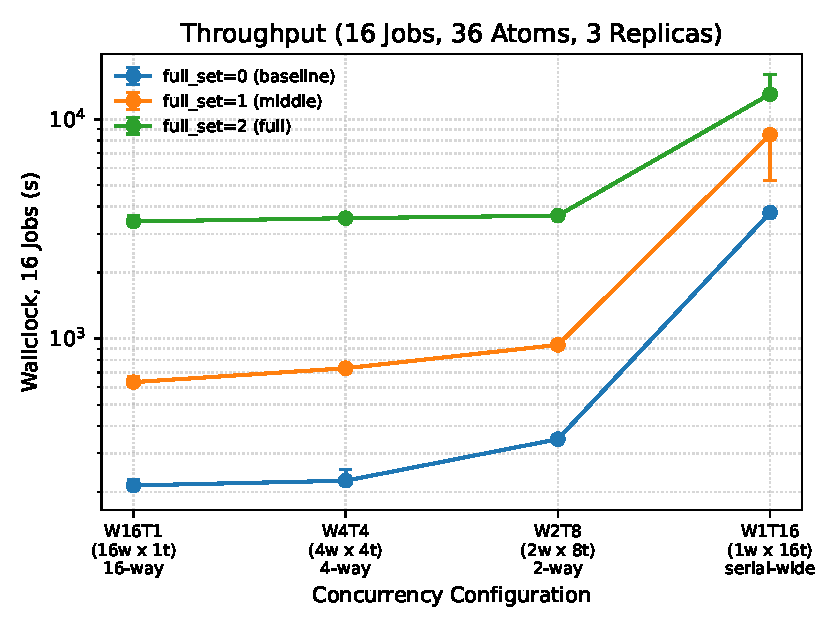
\includegraphics[width=0.75\textwidth]{figures/profiling_study/throughput_curves.pdf}
\caption{Multiwfn QTAIM post-processing wallclock as a function of intra-node concurrency
configuration. Each configuration processes 16 homogeneous copies of \texttt{droplet\_test}
(36 atoms, def2-TZVPD) under cascade-restart tiers. Configurations saturate a 16-thread
budget differently: W16T1 (16 workers $\times$ 1 thread), W4T4 (4 workers $\times$ 4 threads),
W2T8 (2 workers $\times$ 8 threads), W1T16 (1 worker $\times$ 16 threads). Each curve represents
a calculation tier (\texttt{full\_set} 0=baseline, 1=middle, 2=full). Tiers 1 and 2 use
\texttt{--restart} from the prior tier, so per-tier totals are cumulative phase wallclocks.
Markers show medians across 3 replicates with min/max whisker error bars. Y-axis is logarithmic
to visualize the ~75$\times$ range spanning W16T1 tier 0 (fastest) to W1T16 tier 2 (slowest).
Hardware: AMD 7950X (16c/32t). ORCA 6.0.1 (\texttt{shared\_openmpi416}) with system OpenMPI
4.1.2; Multiwfn 3.8 (Oct 2024 dev). ORCA SCF is precomputed; this measures post-processing only.}
\label{fig:throughput_scaling}
\end{figure}


\end{document}

